	% HMC Math dept HW template example
	% v0.04 by Eric J. Malm, 10 Mar 2005
	\documentclass[10pt,a4paper,boxed]{hmcpset}

	% set 1-inch margins in the document
	% \usepackage[margin=1in]{geometry}
	\usepackage{enumerate}
	\usepackage{todonotes}
	\usepackage{tikz}
	\usetikzlibrary{positioning}
	\usepackage{subfig} % subfigures in figures.	
	\usepackage{pgfplots}
	\usepackage{amsmath}
	\usepackage{amsfonts}
	\usepackage{amssymb}
	
	%% work around for subfig and asy environment
	\makeatletter
	\newsavebox{\sfe@box}
	\newenvironment{subfloatenv}[2]{%
	\def\sfe@caption{#1}%
	\def\sfe@label{#2}%
	\setbox\sfe@box\hbox\bgroup\color@setgroup}%
	{\color@endgroup\egroup\subfloat[\sfe@caption]%
	{\usebox{\sfe@box}\label{\sfe@label}}}
	\makeatother

	% include this if you want to import graphics files with /includegraphics
	\usepackage{graphicx}

	\renewcommand*{\familydefault}{\sfdefault}
	\newcommand{\vect}[1]{\mathbf{#1}}
	\newcommand{\Vor}[1]{\textrm{Vor}(#1)}
	\DeclareMathOperator{\gain}{Gain}
	\DeclareMathOperator{\entropy}{H}
	\DeclareMathOperator{\prob}{P}

	\tikzset{node distance=2cm, inner/.style={draw,circle}, leaf/.style={draw,rectangle}}

	% info for header block in upper right hand corner
	\name{Group 6: Timm Behner, Philipp Bruckschen, Patrick Kaster, Markus Schwalb}
	\class{MA-INF 4111 - Intelligent Learning and Analysis Systems: Machine Learning}
	\assignment{Exercise Sheet 4}
	% \duedate{09/03/2004}

	\begin{document}
	
		\begin{problem}[1. Voronoi diagrams]
		\end{problem}

		\begin{solution}		
			\begin{enumerate}[(a)]
				\item Proof by induction over the number of points on a circle with radius $r$ in $\mathbb{R}^2$:
					\begin{description}
						\item[Induction start: $n=3$] Three point lying on a circle with radius $r$ are noncollinear and the resulting cells are unbounded (figure \ref{fig:circ1}).
						\item[Induction step: $n \rightarrow n+1$] Let the induction assumption be true for $n$ points. Let $p, q$ be two abitrary neighboring points on the circle. We insert a new point $o$ exactly at the intersection of the bisector of $p, q$ and the circles radius $r$. The resulting cells are unbounded (figure \ref{fig:circ2}).
					\end{description}
					
					\begin{figure}[h]
  						\centering
  						\begin{subfloatenv}{induction start}{fig:circ1}
  							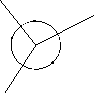
\includegraphics[scale=2]{1ai.pdf} 
  						\end{subfloatenv}
  						\begin{subfloatenv}{induction step}{fig:circ2}
  							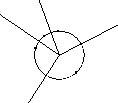
\includegraphics[scale=2]{1aii.pdf} 
  						\end{subfloatenv}
  						\caption{proof by induction over points on a circle}
   						% das label muss immer nach der caption kommen, sonst gibt es Probleme bei der Referenzierung und Nummerierung.
  						\label{fig:circ}
						\end{figure}
				
				\item Let $\Vor{P}$ denote the Voronoi diagram of points $P$. Euler's formula for planer graphs states that
				\[ v - e + f = 2\,, \] where $v, e, f$ denote the number of vertices, edges and faces of the graph.
				
				The number of faces is $ f = \vert P \vert = n = \#\textrm{cells } (\Vor{P})$. To make use of Euler's formula, we have to construct a planar Graph from $ \Vor{P} $, by adding an additional vertex to the diagram, situated at infinity, and connecting every infinite edge (from the unbounded cells) to this vertex (figure \ref{fig:VorGraph}).
				
				\begin{figure}[h]
    			\centering
    			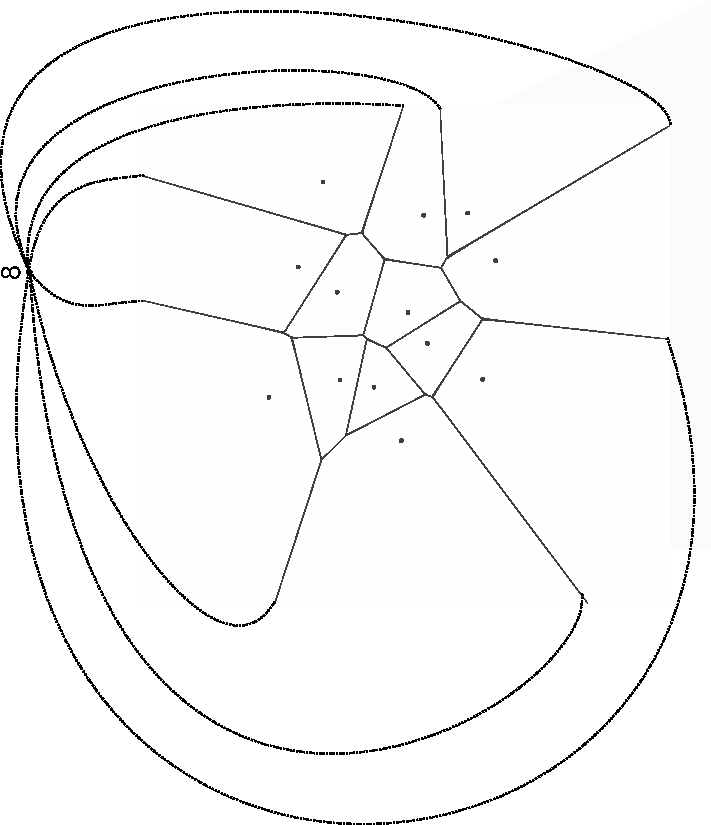
\includegraphics[scale=0.3]{1b.pdf} 
    			\caption{augmenting Voronoi diagram to planar graph}
    			\label{fig:VorGraph}
				\end{figure} 
				
				We note that each edge in $ \Vor{P} $ has exactly two incident vertices and each vertex of $ \Vor{P}+\infty $ has at least degree (\textrm{deg}) $ 3 $. Therefore we conclude
				\begin{align}
					\sum_{\textrm{vertex} \in \Vor{P}+\infty} \textrm{deg}(\textrm{vertex})  = 2e \geq 3 (v + 1) \label{eq:1}
				\end{align}
								
				Since we inserted our additional point $ \infty $, Euler's Formula for our constructed graph is:
				\[ (v+1)-e+f = (v+1)-e+n = 2 \]
				Inserting this into (\ref{eq:1}) gives us:
				\begin{alignat*}{2}
					2 e &\geq 3 (2 + e - n) = 6 + 3e - 3n \Rightarrow \\
					 e & \leq 3n - 6
				\end{alignat*}
				Inserting this result into (\ref{eq:1}):				
				\begin{alignat*}{2}
					v & \leq 2n - 5
				\end{alignat*}
				
									 
				
			\end{enumerate}
			
		\end{solution}		


	\end{document}
